%% =====================================================================
%%  ELL305 Project Report -- single-file LaTeX template (LIPIcs-inspired)
%%  Author : Olivia
%%  Build  : pdflatex -> bibtex -> pdflatex -> pdflatex
%%           (or simply: latexmk -pdf <file>.tex ; Overleaf does this automatically)
%%  Rules covered: single .tex file, A4, 1 inch margins, 12pt, single spacing,
%%  double-sided, TikZ diagrams, listings for code, auto TOC / LOF / LOT,
%%  glossary, index, copyright on page 2, acknowledgements on page 3,
%%  Appendix A = plagiarism report, Appendix B = readability indices.
%% =====================================================================

%% ---------- Bibliography (export from Zotero as BibTeX and paste here) ----------
\begin{filecontents*}[overwrite]{\jobname.bib}
@book{sarangi,
  author    = {Smruti R. Sarangi},
  title     = {Basic Computer Architecture},
  publisher = {White Falcon Publishing},
  year      = {2021},
  note      = {Video lectures for each chapter by the author are available on YouTube}
}
@manual{ug585,
  title        = {Zynq-7000 SoC Technical Reference Manual (UG585)},
  organization = {AMD Xilinx},
  year         = {2023}
}
@manual{axispec,
  title        = {AMBA AXI and ACE Protocol Specification (IHI 0022)},
  organization = {Arm Limited},
  year         = {2021}
}
@manual{zybo,
  title        = {Zybo Z7 Reference Manual},
  organization = {Digilent},
  year         = {2023}
}
@book{burden,
  author    = {Richard L. Burden and J. Douglas Faires},
  title     = {Numerical Analysis},
  edition   = {9th},
  publisher = {Brooks/Cole},
  year      = {2011}
}
\end{filecontents*}

\documentclass[12pt,a4paper,twoside]{article}

%% ---------- Page layout: A4, 1 inch margins, single spacing ----------
\usepackage[a4paper,margin=1in,headheight=15pt]{geometry}
\usepackage[T1]{fontenc}
\usepackage[utf8]{inputenc}
\usepackage{lmodern}
\usepackage{microtype}

%% ---------- Colours (LIPIcs-like yellow and greys) ----------
\usepackage[table]{xcolor}
\definecolor{lipicsyellow}{RGB}{247,201,49}
\definecolor{lipicsgray}{RGB}{90,90,90}
\definecolor{lipicslight}{RGB}{245,245,245}
\definecolor{codekw}{RGB}{0,60,140}
\definecolor{codecm}{RGB}{90,120,90}

%% ---------- Headings: sans-serif bold, section number in a yellow box ----------
\usepackage{titlesec}
\titleformat{\section}
  {\sffamily\bfseries\Large}
  {\colorbox{lipicsyellow}{\strut\hspace{0.15em}\thesection\hspace{0.15em}}}
  {0.7em}{}
\titleformat{\subsection}
  {\sffamily\bfseries\large}{\thesubsection}{1em}{}
\titleformat{\subsubsection}
  {\sffamily\bfseries\normalsize}{\thesubsubsection}{1em}{}
\titlespacing*{\section}{0pt}{3.0ex plus 1ex minus .2ex}{1.6ex plus .2ex}

%% ---------- Running header: page number + short title / author ----------
\usepackage{fancyhdr}
\newcommand{\shorttitle}{RK4 Integration Accelerator on the Zynq-7020}
\newcommand{\shortauthor}{Olivia}
\pagestyle{fancy}
\fancyhf{}
\fancyhead[LE]{\sffamily\bfseries\thepage\qquad\shorttitle}
\fancyhead[RO]{\sffamily\bfseries\shortauthor\qquad\thepage}
\renewcommand{\headrulewidth}{0pt}
\fancypagestyle{plain}{\fancyhf{}\fancyfoot[C]{\sffamily\thepage}\renewcommand{\headrulewidth}{0pt}}

%% ---------- Lists: small grey bars as bullets (LIPIcs style) ----------
\usepackage{enumitem}
\setlist[itemize,1]{label=\textcolor{lipicsgray}{\rule[0.35ex]{1.1ex}{0.55ex}}}
\setlist[itemize,2]{label=\textcolor{lipicsgray}{\rule[0.45ex]{0.8ex}{0.35ex}}}
\setlist{itemsep=0.2ex,topsep=0.6ex}

%% ---------- Floats, tables, captions ----------
\usepackage{graphicx}
\usepackage{booktabs}
\usepackage{tabularx}
\usepackage{array}
\usepackage[labelfont={sf,bf},font=small]{caption}
\usepackage{float}
\usepackage{siunitx}

%% ---------- Diagrams (TikZ) ----------
\usepackage{tikz}
\usetikzlibrary{positioning,arrows.meta,shapes.geometric,fit,calc}
\tikzset{
  blk/.style={draw,rounded corners=2pt,fill=lipicslight,minimum height=9mm,
              minimum width=26mm,align=center,font=\sffamily\small},
  hl/.style={blk,fill=lipicsyellow!45},
  arr/.style={-{Stealth[length=2.5mm]},thick}
}

%% ---------- Code listings ----------
\usepackage{listings}
\lstdefinestyle{report}{
  basicstyle=\ttfamily\footnotesize,
  keywordstyle=\color{codekw}\bfseries,
  commentstyle=\color{codecm}\itshape,
  backgroundcolor=\color{lipicslight},
  frame=single, rulecolor=\color{lipicsgray!40},
  numbers=left, numberstyle=\tiny\color{lipicsgray}, numbersep=6pt,
  breaklines=true, showstringspaces=false, tabsize=4,
  captionpos=b, xleftmargin=1.5em, framexleftmargin=1.5em
}
\lstset{style=report}
\renewcommand{\lstlistlistingname}{List of Listings}

%% ---------- Index and glossary (no external tools needed for the glossary) ----------
\usepackage{imakeidx}
\makeindex[intoc,columns=2]
\usepackage[hidelinks]{hyperref}
\hypersetup{colorlinks=true,linkcolor=black,citecolor=codekw,urlcolor=codekw}
\usepackage[toc,nonumberlist]{glossaries}
\makenoidxglossaries

%% ---------- Glossary entries (add more as you write) ----------
\newacronym{axi}{AXI}{Advanced eXtensible Interface, Arm's on-chip bus protocol (AMBA family)}
\newacronym{pl}{PL}{Programmable Logic, the FPGA fabric of the Zynq}
\newacronym{ps}{PS}{Processing System, the ARM processor side of the Zynq}
\newacronym{uart}{UART}{Universal Asynchronous Receiver/Transmitter}
\newacronym{rk4}{RK4}{fourth-order Runge--Kutta method}
\newacronym{dsp}{DSP}{dedicated multiply--accumulate block (DSP48E1) in the FPGA}
\newacronym{wns}{WNS}{Worst Negative Slack, the timing margin reported by Vivado}
\newacronym{bsp}{BSP}{Board Support Package, the low-level software library in Vitis}
\newglossaryentry{polling}{name={polling},description={a processor repeatedly reading a device's status register until the device reports that it has finished}}
\newglossaryentry{qformat}{name={Q-format},description={fixed-point notation; Q16.16 means 16 integer bits and 16 fractional bits in a 32-bit two's-complement word}}
\newglossaryentry{hazard}{name={data hazard},description={a pipeline conflict in which an operation needs a result that is not yet available}}

%% ---------- Handy macros ----------
\newcommand{\todo}[1]{{\sffamily\footnotesize\colorbox{lipicsyellow!60}{TODO}\ \textcolor{lipicsgray}{#1}}}
\newcommand{\file}[1]{\texttt{#1}}

%% =====================================================================
\begin{document}

%% ---------------------------- Page 1: Title ----------------------------
\begin{titlepage}
\centering
\vspace*{\fill}
{\sffamily\bfseries\Huge ELL305 -- Project Report\par}
\vspace{3mm}
{\large\itshape Draft \#1 of 4 : Progress Report\par}
\vspace{4mm}
\textcolor{lipicsyellow}{\rule{0.35\linewidth}{1.2mm}}\par
\vspace{6mm}
{\sffamily\bfseries\Large A Pipelined RK4 Integration Accelerator\\
on the Zynq-7020 with\\
Logic-Analyser-Verified Interfacing\par}
\vspace{10mm}
{\sffamily\bfseries\LARGE Olivia\par}
\vspace{2mm}
{\large\bfseries 2024MT10925\par}
\vspace{2mm}
{\large\itshape \today\par}
\vspace{10mm}
{\large Department of Electrical Engineering\\
Indian Institute of Technology Delhi\par}
\vspace*{\fill}
\begin{tikzpicture}[remember picture,overlay]
  \fill[lipicsyellow] ([xshift=-60mm,yshift=26mm]current page.south east) rectangle ([yshift=18mm]current page.south east);
\end{tikzpicture}
\end{titlepage}

%% ---------------------------- Page 2: Copyright ----------------------------
\thispagestyle{empty}
\vspace*{\fill}
\begin{center}
  {\sffamily\bfseries\large Copyright \textcopyright\ 2026 by Olivia\par}
  \vspace{1.2em}
  \begin{minipage}{0.78\linewidth}
    \centering
    All Intellectual Property Rights (IPR) associated with this technical report and its
    primary designs belong to the \textbf{Indian Institute of Technology Delhi}.
    In the case of cited material, IPR belongs to the respective authors and sources referenced.
  \end{minipage}
  \vspace{2.5em}

  \textcolor{lipicsyellow}{\rule{0.25\linewidth}{1.2mm}}
\end{center}
\vspace*{\fill}
\newpage

%% ---------------------------- Page 3: Acknowledgements ----------------------------
\thispagestyle{empty}
\vspace*{8mm}
{\sffamily\bfseries\LARGE Acknowledgement\par}
\vspace{1mm}
\textcolor{lipicsyellow}{\rule{\linewidth}{1.2mm}}
\vspace{6mm}

I sincerely thank the course instructors, \textbf{Prof.~Subrat Kar} and
\textbf{Prof.~Sumantra Dutta Roy}, for their guidance, encouragement and support throughout
the course and the project. I am especially grateful for the opportunity to study Computer
Architecture and to work on this project, which gave me valuable hands-on experience and
allowed me to apply the concepts learned in class to gain a deeper and more practical
understanding of the subject.

I would also like to sincerely thank the Teaching Assistants, in particular
\textbf{Utkarsh Roy} and \textbf{Deepak Priyadarshi}, for their constant assistance, for
patiently clarifying my doubts, for helping me with the experiments on the Zybo board and the
logic analyser, and for reviewing my progress throughout the project.

I gratefully acknowledge the \textbf{Department of Electrical Engineering} and the
\textbf{Indian Institute of Technology Delhi} for providing the laboratory facilities,
equipment, software and computing resources that made this work possible.

\vspace{12mm}
\noindent{\sffamily\bfseries Olivia}\\
\today
\newpage

%% ---------------------------- Lists ----------------------------
\tableofcontents
\listoffigures
\listoftables
\lstlistoflistings
\newpage

%% =====================================================================
\section{Introduction}

\subsection{Relevance to ELL305}

\subsubsection*{Chapters from \emph{Basic Computer Architecture} (S.~R.~Sarangi) this project draws upon}
This project is based on the course textbook, \emph{Basic Computer Architecture} by
Smruti R.~Sarangi~\cite{sarangi}. Its main basis is \textbf{Chapter~13, I/O and Storage Devices},
because the project is a processor controlling a custom peripheral over a bus and exchanging data
with the user over a serial link. The design of the peripheral itself draws on several earlier
chapters, as summarised in Table~\ref{tab:chapters}.

\begin{table}[H]
\centering
\caption{Chapters of the textbook~\cite{sarangi} used in this project.}
\label{tab:chapters}
\small
\begin{tabularx}{\linewidth}{@{}>{\raggedright\arraybackslash\hyphenpenalty=10000}p{0.31\linewidth}X@{}}
\toprule
\textbf{Chapter} & \textbf{Where it appears in the project} \\
\midrule
\multicolumn{2}{@{}l}{\textbf{Main basis}} \\
\textbf{13 -- I/O and Storage Devices}, Part~I (physical layer)
  & Asynchronous \gls{uart}\index{UART} link at 115200 baud, 8N1 framing (start bit, 8 data bits, stop bit), no shared clock; frames observed and decoded with a logic analyser. \\
\textbf{13}, Part~II (data link, network and protocol layers)
  & Memory-mapped registers on the \gls{axi}4-Lite\index{AXI4-Lite} bus; the processor writes inputs and a start command, then detects completion by \gls{polling}\index{polling} a status register (programmed I/O); VALID/READY handshakes. \\
\textbf{13}, Part~III (USB)
  & Programming and the serial terminal pass through the board's USB interface. \\
\midrule
\multicolumn{2}{@{}l}{\textbf{Supporting material}} \\
\textbf{2 -- Language of Bits}
  & Fixed-point two's-complement numbers (\gls{qformat}: Q16.16 and Q1.23) instead of floating point. \\
\textbf{7 -- Digital Logic}
  & Registers (flip-flops) separating the combinational stages of the datapath. \\
\textbf{8 -- Computer Arithmetic}
  & Hardware integer multipliers and adders (\gls{dsp} blocks), with rounding after each multiplication. \\
\textbf{10 -- Principles of Pipelining}
  & A ten-stage RK4 pipeline; the \gls{hazard} between consecutive steps is avoided by interleaving ten independent equations per pipeline. \\
\textbf{11 -- Memory System}
  & The accelerator's registers occupy part of the processor's address space; cache warm-up affects the measured software time. \\
\textbf{12 -- Multiprocessor Systems}
  & Two pipelines work in parallel on twenty data sets, in the spirit of vector (SIMD) processing. \\
\bottomrule
\end{tabularx}
\end{table}

\subsection{Significance of the Project}

\subsubsection*{Concepts from the textbook my project illustrates}

\paragraph{Central idea: Input/Output Interfacing (Chapter~13: I/O and Storage Devices).}
This project illustrates how a processor communicates with an external device through
well-defined interface layers, and how that communication can be observed and verified at the
signal level. Instead of using an off-the-shelf peripheral, I designed my own: a hardware
accelerator that solves ordinary differential equations of the form
$\mathrm{d}y/\mathrm{d}x = a\,y + b\,x + c$ with the fourth-order Runge--Kutta (\gls{rk4}) method.
It is implemented in the programmable logic of a Zynq-7020 and attached to the on-chip ARM
Cortex-A9 processor, while the serial link uses the processor's built-in \gls{uart} controller.

% NOTE: "how far the solution is advanced" (not "accurate"): with a fixed step size h,
% the number of steps sets the end point x = steps * h, not the accuracy.
The user selects one of five preset equations from a menu and enters the number of integration
steps, which sets how far the solution is advanced ($x = \text{steps} \times h$, with $h = 0.01$).
At the protocol layer, the accelerator appears to the processor as memory-mapped registers on the
\gls{axi}4-Lite\index{AXI4-Lite} bus. For each run, the processor writes the chosen equation's
coefficients, twenty fixed starting values and the number of steps into these registers, issues a
start command, and polls a status register until the device has finished. This is programmed I/O
by \gls{polling}\index{polling}, and its cost is visible: while waiting, the processor does no
useful work, which is the trade-off the chapter uses to motivate interrupts and DMA. At the
physical and data-link layers, the user communicates with the board over an asynchronous UART
link\index{UART} at 115200 baud with 8N1 framing: each character is carried by a start bit, eight
data bits and a stop bit, without a shared clock. A logic analyser shows these frames on the wire
and decodes them back into the commands sent and the results returned.

The project also shows how interfaces support measurement. The accelerator and the processor each
drive a general-purpose output pin while computing, and the pulse widths captured by the logic
analyser provide their execution times independently of any software timer. This confirmed that
the hardware takes exactly ten clock cycles per integration step, as designed, and completes the
same workload [X] times faster than the processor.

\paragraph{Supporting concepts from Chapters 1--12.}
The accelerator itself applies earlier chapters. Numbers use fixed-point two's-complement form
(Chapter~2: Language of Bits), and the datapath is built from registers separating combinational
stages (Chapter~7: Digital Logic). Each step uses hardware multipliers and adders with rounding
(Chapter~8: Computer Arithmetic). The datapath is a ten-stage pipeline (Chapter~10: Principles of
Pipelining). Since each RK4 step depends on the previous one, a \gls{hazard} that would normally
stall the pipeline is avoided by interleaving ten independent equations per pipeline, producing
one result per clock cycle. Two pipelines work in parallel on twenty data sets, in the spirit of
vector processing (Chapter~12: Multiprocessor Systems), and the accelerator's registers occupy
part of the processor's address space (Chapter~11: Memory System).

The project thus connects the inside of a device (pipelining and arithmetic) with the way it is
attached to, controlled by and verified from a processor, the central theme of Chapter~13.

\subsection{Objectives}
The project had six objectives. Each one has a measurable criterion, listed in brackets, which is
checked in Sections~\ref{sec:verification} and~\ref{sec:results}.
\begin{enumerate}[label=\textbf{O\arabic*.},leftmargin=3em]
  \item \textbf{Design the accelerator.} Build a pipelined, fixed-point \gls{rk4} datapath in Verilog
        for $\mathrm{d}y/\mathrm{d}x = a\,y + b\,x + c$ that solves twenty starting values in parallel
        in the programmable logic of the Zynq-7020.
        \emph{(One integration step per clock cycle per pipeline at 100\,MHz, with \gls{wns}~$\geq 0$.)}
  \item \textbf{Interface it to the processor.} Connect the accelerator to the ARM Cortex-A9 as a
        memory-mapped \gls{axi}4-Lite peripheral that the processor configures, starts and
        monitors by \gls{polling}.
        \emph{(The processor reads the correct identification register and receives results for every run.)}
  \item \textbf{Provide user input and output.} Let the user choose one of five preset equations
        and the number of steps over a \gls{uart} link, and print the results and run times.
        \emph{(Menu, input and results work through a serial terminal and the logic analyser.)}
  \item \textbf{Verify correctness.} Check the hardware against a bit-exact fixed-point model and
        against double-precision software.
        \emph{(All twenty results bit-exact in simulation and on hardware; difference from
        double precision of the order of $10^{-4}$.)}
  \item \textbf{Measure performance independently.} Expose the busy periods of the accelerator and
        the processor on output pins and measure them with a logic analyser.
        \emph{(Pulse width of ten clock cycles per step; speed-up over the processor quantified.)}
  \item \textbf{Document the work for continuation.} Record every design decision, every problem
        encountered and its fix, and the full build procedure.
        \emph{(A new person can rebuild and run the project from this report alone.)}
\end{enumerate}

\subsection{Organisation of this Report}
\todo{one sentence per section.}

%% =====================================================================
\section{Background}
\subsection{The Fourth-Order Runge--Kutta Method}
\todo{one paragraph; the full derivation goes to Appendix~\ref{app:rk4}.} \cite{burden}
\subsection{The Zynq-7020 Platform}
\todo{\gls{ps} vs \gls{pl}, Cortex-A9, Zybo Z7-20} \cite{ug585,zybo}
\subsection{AXI4-Lite and Memory-Mapped I/O}
\todo{five channels, VALID/READY handshake.}
\subsection{UART and 8N1 Framing}
\todo{start bit, 8 data bits, stop bit; no shared clock.}

%% =====================================================================
\section{System Architecture}
Figure~\ref{fig:system} shows the complete system.

\begin{figure}[H]
\centering
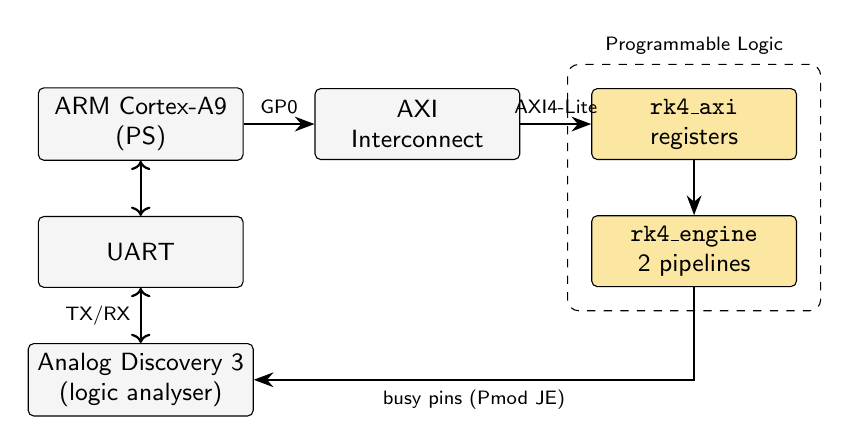
\begin{tikzpicture}[node distance=7mm and 9mm]
  \node[blk] (arm) {ARM Cortex-A9\\(PS)};
  \node[blk,right=of arm] (ic) {AXI\\Interconnect};
  \node[hl,right=of ic] (acc) {\texttt{rk4\_axi}\\registers};
  \node[hl,below=of acc] (eng) {\texttt{rk4\_engine}\\2 pipelines};
  \node[blk,below=of arm] (uart) {UART};
  \node[blk,below=of uart] (ad3) {Analog Discovery 3\\(logic analyser)};
  \draw[arr] (arm) -- node[above,font=\scriptsize\sffamily]{GP0} (ic);
  \draw[arr] (ic) -- node[above,font=\scriptsize\sffamily]{AXI4-Lite} (acc);
  \draw[arr] (acc) -- (eng);
  \draw[arr,<->] (arm) -- (uart);
  \draw[arr,<->] (uart) -- node[left,font=\scriptsize\sffamily]{TX/RX} (ad3);
  \draw[arr] (eng.south) |- node[pos=0.75,below,font=\scriptsize\sffamily]{busy pins (Pmod JE)} (ad3.east);
  \node[draw,dashed,rounded corners,inner sep=3mm,fit=(acc)(eng),
        label={[font=\scriptsize\sffamily]above:Programmable Logic}] {};
\end{tikzpicture}
\caption{System overview (example TikZ diagram -- edit to match the final design).}
\label{fig:system}
\end{figure}

\begin{table}[H]
\centering
\caption{Accelerator register map (base address \texttt{0x43C00000}).}
\label{tab:regmap}
\small
\begin{tabular}{@{}lll@{}}
\toprule
\textbf{Offset} & \textbf{Name} & \textbf{Meaning} \\
\midrule
\texttt{0x00} & CTRL   & write 1 = start \\
\texttt{0x04} & STATUS & bit 0 done, bit 1 busy \\
\texttt{0x08} & STEPS  & number of RK4 steps \\
\texttt{0x18} & CYCLES & clock cycles of the last run \\
\texttt{0x1C} & ID     & reads \texttt{0x524B3402} \\
\texttt{0x80}--\texttt{0xCC} & Y[0..19] & Q16.16 values \\
\bottomrule
\end{tabular}
\end{table}
\todo{complete the table; full details in Appendix~\ref{app:regs}.}

%% =====================================================================
\section{Hardware Design}
\subsection{The RK4 Pipeline (\file{rk4\_core.v})}\todo{}
\subsection{Data Hazards and Interleaving}
\todo{explain; timing diagram drawn with WaveDrom (see note below).}

\begin{figure}[H]
\centering
\IfFileExists{wavedrom_interleave.pdf}
  {\includegraphics[width=0.9\linewidth]{wavedrom_interleave.pdf}}
  {\fbox{\parbox{0.8\linewidth}{\centering\sffamily\small WaveDrom figure goes here\\
   (render the WaveDrom JSON in Appendix~\ref{app:code} to \file{wavedrom\_interleave.pdf})}}}
\caption{Interleaving of ten equations through one pipeline (WaveDrom).}
\label{fig:interleave}
\end{figure}

\subsection{Engine and AXI4-Lite Wrapper}\todo{}
\subsection{Timing Pins}\todo{}
\subsection{Implementation Results}\todo{utilisation table, \gls{wns} at 100\,MHz.}

%% =====================================================================
\section{Design Decisions}
\begin{table}[H]
\centering
\caption{Summary of design decisions (each explained in its own subsection).}
\label{tab:decisions}
\small
\begin{tabularx}{\linewidth}{@{}lX@{}}
\toprule
\textbf{\#} & \textbf{Decision, alternatives and reason} \\
\midrule
D1 & \todo{} \\
D2 & \todo{} \\
\bottomrule
\end{tabularx}
\end{table}

%% =====================================================================
\section{Software Design}
The core of the polling loop is shown in Listing~\ref{lst:poll}.
\begin{lstlisting}[language=C,caption={Starting the accelerator and polling its status register.},label={lst:poll}]
wr(REG_CTRL, 1);                      /* start                     */
while (!(rd(REG_STATUS) & 1)) ;       /* poll until bit 0 (done)   */
\end{lstlisting}
\todo{flowchart (TikZ), BSP settings (\gls{bsp}), bit-exact model.}

%% =====================================================================
\section{Verification in Simulation}\label{sec:verification}\todo{golden model, testbench, results table.}
\section{Hardware Results}\label{sec:results}\todo{setup photo, accuracy table, pulse widths, speed-up.}
\section{Problems Encountered and Lessons Learned}\todo{table: problem, cause, fix.}
\section{Current Status and How to Continue}\todo{what works, files, rebuild steps, next steps.}
\section{Conclusion and Future Work}\todo{}

%% =====================================================================
\bibliographystyle{plain}
\bibliography{\jobname}

%% =====================================================================
\appendix
\section{Plagiarism Report}\label{app:plag}
\todo{attach the Turnitin report; it must match the submission on turnitin.com.}

\section{Readability Indices}\label{app:read}
\begin{table}[H]
\centering
\caption{Readability indices of this report.}
\label{tab:readability}
\begin{tabular}{@{}lr@{}}
\toprule
\textbf{Index} & \textbf{Score} \\
\midrule
Flesch Reading Ease & \todo{} \\
Flesch--Kincaid Grade Level & \todo{} \\
Gunning Fog Index & \todo{} \\
SMOG Index & \todo{} \\
Coleman--Liau Index & \todo{} \\
Automated Readability Index & \todo{} \\
\bottomrule
\end{tabular}
\end{table}

\section{Derivation of RK4 for dy/dx = a\,y + b\,x + c}\label{app:rk4}\todo{}
\section{Full Register Map and AXI4-Lite Details}\label{app:regs}\todo{}
\section{Source Code}\label{app:code}
\todo{full Verilog, C, Python and Tcl listings, and the WaveDrom JSON sources.}

%% =====================================================================
\clearpage
\printnoidxglossaries
\printindex

\end{document}
